Эксперименты ставились на парах модельных изображений и на изображениях поверхностях реальных образцов.

\subsection{Модельные изображения}

В качестве образцов брались наборы изображений из интернет ресурса ``Society for Experimental Mechanics (sem.org)'' описание текстур находится в таблице \ref{tab:set_image}.

\begin{longtable}[h!]{|*7{m{0.12\textwidth}|}}
\caption{Описание используемых серий изображений}
\label{tab:set_image}
\\ \hline
Серия & Имя & Метод & Диапазон яркостей 	& Уровень шума & Сдвиг (px) & Кол-во изображений \\ \hline
Grey texture & Grey set & Shift  & 0-188 & Нет & 1-20 & 5   \\ \hline
HC texture & High contrast & QEM & 10-240 & Низкий  & 0.1-1 & 122  \\ \hline
Prosilica Bin  & Sample6  & Binning & 10-156 & Низкий  & 0.1-1 & 10   \\ \hline
Strain Gradient & Sample11b & FFT & 20-185 	& Средний  & 0.01-1  & 6   \\ \hline
Strain Gradient & Sample10  & FFT & 30-225 	& Средний  & 0.01-1  & 10   \\ \hline
\end{longtable}

\begin{figure}[ht]
\center{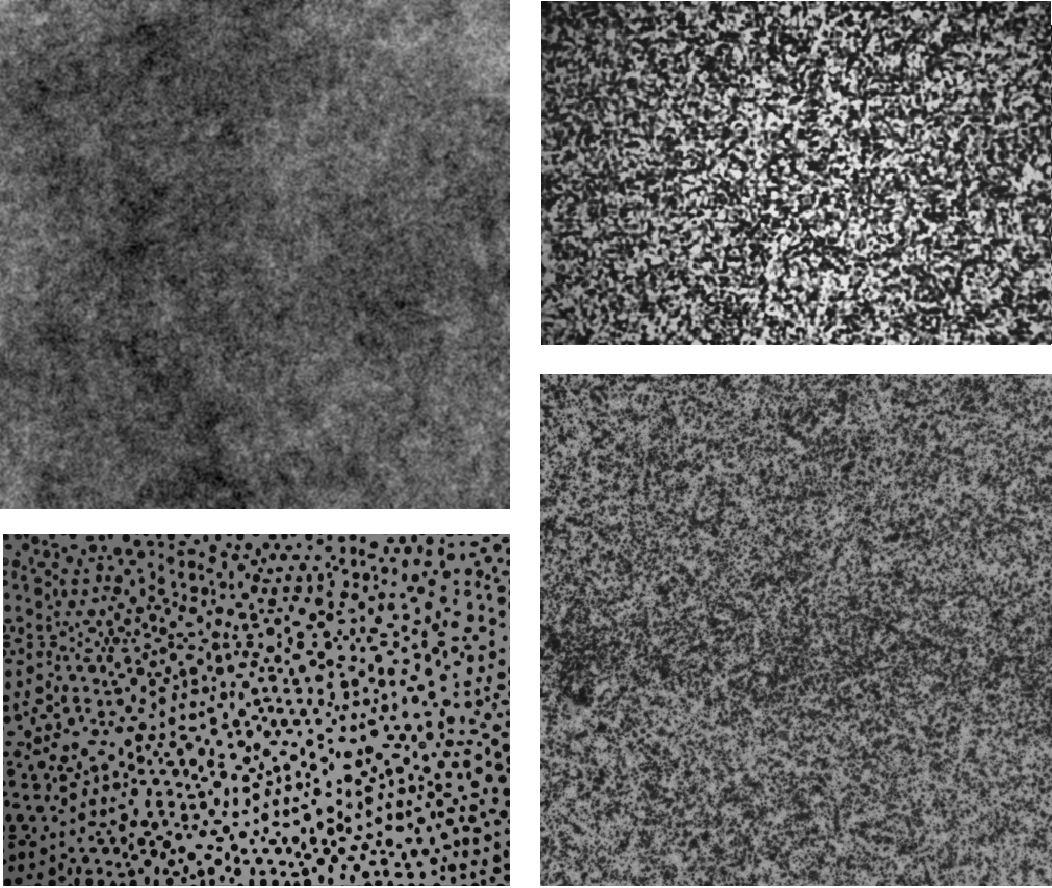
\includegraphics[width=0.8\linewidth]{gray_mix}}
\caption{Тестовая серия изображений: По часовой стрелке Серая подборка, Тестовая серия №11, Серия высокого контраста, Тестовая серия №6}
\label{pic:gray_mix}
\end{figure}

\begin{figure}[ht]
\center{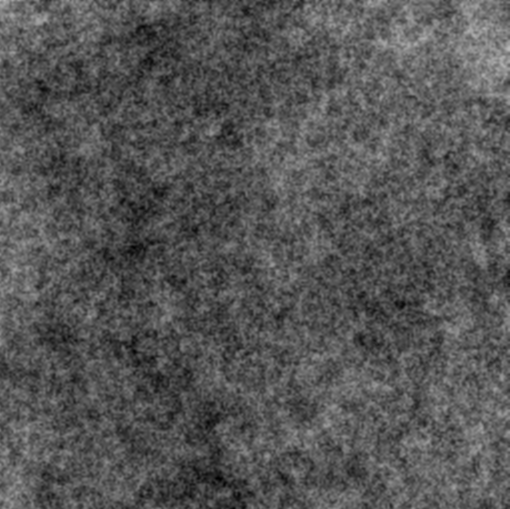
\includegraphics[width=0.8\linewidth]{gray_set}}
\caption{Тестовая серия изображений:Grey texture}
\label{pic:gray_set}
\end{figure}

\subsection{Реальные отснятые изображения}

В данном разделе приведены результаты тестирования разрабатываемого программного обеспечения на изображениях поверхностей реальных образцов. В экспериментах использовались металлические образцы из авиационного алюминиевого сплава Д16АТ и полимерные образцы из полипропилена, нагружавшиеся на механической испытательной машине ИМАШ-2078 в условиях одноосного статического растяжения.

\begin{figure}[ht]
\center{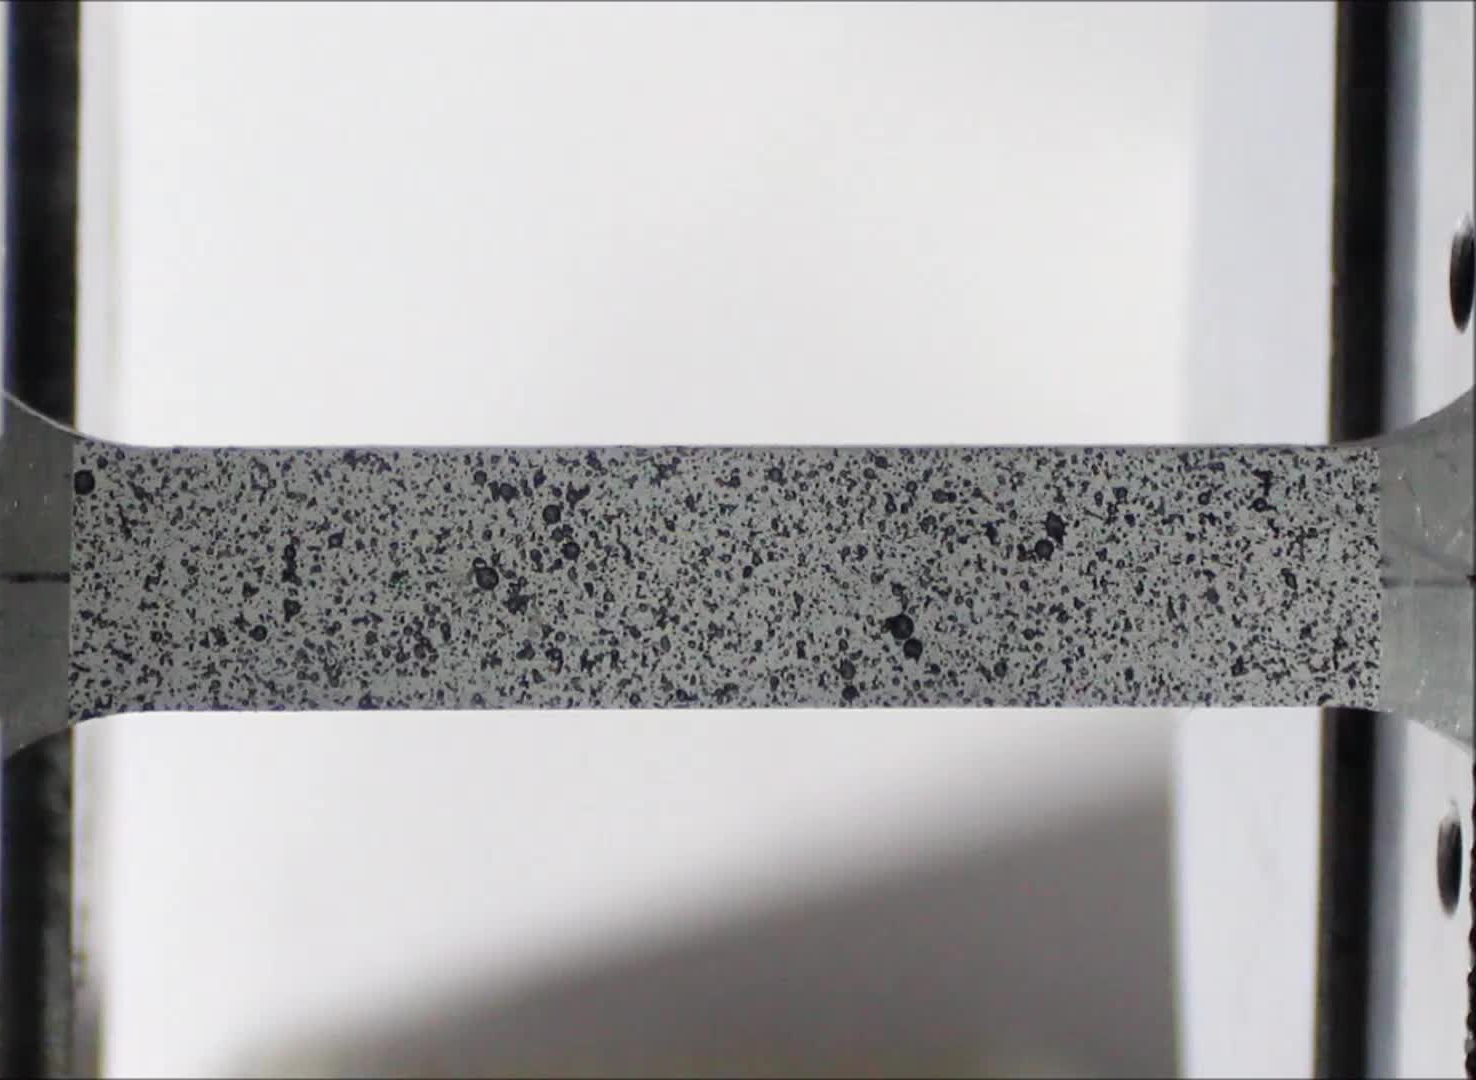
\includegraphics[width=0.6\linewidth]{real_deform}}
\caption{Растяжение пластины алюминия Д16АТ}
\label{pic:real_deform}
\end{figure}

\subsection{Синтетические изображения}

Для первого раза используем изображения из серии Grey texture, представленные на рисунке \ref{pic:gray_set}. Они имеют сдвиг по оси $x$ на один пиксель влево, по $y$ сдвиг отсутствует.


\subsection{Экспериментальные изображения}